\documentclass[12pt,a4paper]{article}
\usepackage[spanish]{babel}
\selectlanguage{spanish}
\usepackage{amsmath}
\usepackage{amsthm}
\usepackage{amsfonts}
\usepackage{amssymb}
\usepackage{multirow}
\usepackage{multicol}
\usepackage[graphicx]{realboxes}
\usepackage[spanish]{babel}
\usepackage{graphicx}
\usepackage[table]{xcolor}
\usepackage{wrapfig}
\usepackage{float} 
\usepackage{xurl} 
\usepackage[margin=3.5cm]{geometry}
\hyphenation{Re-fe-ren-cias}
\usepackage{fancyhdr}
%\usepackage{color}              % For creating coloured text and background
\usepackage[hidelinks]{hyperref}            % For creating hyperlinks in cross references
\columnsep 0.8 cm
\pagestyle{plain}
\newtheorem{teorema}{Teorema}
\fancyfoot{}

\begin{document}
\renewcommand{\tablename}{Tabla}
\renewcommand{\refname}{Referencias bibliográficas}

\begin{titlepage}

\vspace*{-3cm}

%\thispagestyle{empty}

{\bf
\begin{center}
\large
\vspace*{-1 cm}\Large \textsc{Universidad Nacional del Este} \\
\Large \textsc{Facultad Politécnica} \\
\vspace*{0.5 cm}\hrule
\vspace*{0.5 cm}
\vspace*{0 cm}\Large Anteproyecto de  Trabajo Final de Grado\\
\vspace*{0.5 cm}\large Carrera Ingeniería de Sistemas\\
\vspace*{0 cm}\large Cátedra Trabajo Final de Grado I\\
\end{center}
}

\vspace{2 cm}
{
\noindent
\begin{center}
\huge \bf Implementación de una estrategia de gamificación en una plataforma virtual de educación para el aprendizaje de la Física
\end{center}
}

\vspace{0.5 cm}

{ 
Por: \textbf{\Large Yudith Gonzalez Mareco}

\hspace{1 cm} y \textbf{\Large Yisell Magalí Rolón Raviolo}

\vspace*{.5 cm}
Profesor Orientador: \textbf{\large Lic. Celso Alberto Rojas Pukall }
}%\\[6mm]
\vspace*{0.5 cm}\\

Profesor de la Cátedra: \textbf{\large Lic. Roberto Alfredo Demestri Rigoni}

\vspace{3.0cm}

\begin{minipage}{0.9\textwidth}
\begin{flushleft}
\begin{footnotesize}
\begin{scriptsize}\end{scriptsize}Tel: 0972 845 554,\\
correo electrónico: yudith199616gonza@gmail.com \\
\vspace*{.5cm}
\begin{scriptsize}\end{scriptsize}Tel: 0985 170 172,\\
 correo electrónico: ravioloyisell5@gmail.com  \\
\vspace*{.5cm}

 \end{footnotesize}
\end{flushleft}
\end{minipage}

\vspace{2.0cm}

\begin{center}
{\large {\bf Ciudad del Este, Alto Paraná - Paraguay}\\[6mm]
\today}\\
\end{center}


\end{titlepage}

\tableofcontents

\vspace{1cm}

\title{Implementación de una estrategia de gamificación en una plataforma virtual de educación para el aprendizaje de la Física}
\vspace{1cm}
\date{}
\maketitle

\thispagestyle{empty}
\section{Definición del problema}
 \textit{Debido al bajo rendimiento que poseen los postulantes para el curso de admisión a las carreras de ingeniería de la FPUNE, en los exámenes de Física, se plantea una propuesta didáctica como estrategia novedosa, apoyada en el uso de los recursos tecnológicos en la que se aplica la gamificación en el proceso de aprendizaje, a través de una plataforma educativa que persigue ayudar a los mismos aumentando su motivación y su interés por aprender, teniendo en cuenta las competencias claves, los contenidos y los objetivos que se especifican en el programa de estudio.}.

\section{Delimitación del trabajo.}


\section{Objetivos}
Diseñar una propuesta didáctica en la que se aplique la gamificación en el proceso de aprendizaje de la física con la practica de una nueva metodología de aprendizaje llamada gamificación con el fin de contribuir en una mejora del aprendizaje de los postulantes.

\subsection{Objetivo general}
Implementar un cambio metodológico para aprovechar los recursos tecnológicos que además favorecerán la motivación del alumnado hacia el área de Física con una propuesta innovadora de gamificación.
 
\subsection{Objetivos específicos}

\begin{enumerate}
\item Desglosar conceptos de física mediante ejercicios concretos orientados a metas definidas.
\item Adaptar la plataforma moodle que refuerce la adquisición de conocimientos científicos por parte de los postulantes.
\item Fomentar el interés de los estudiantes en la materia a través de una representación dinámica, interactiva y divertida de los temas.
\item Establecer rankings para indicar progresión-, trayectorias- y desempeño académico generado dentro del proyecto gamificado propuesto, orientado al temario curricular en cuestión.\\


\end{enumerate}

\section{Hipótesis}
Para el método científico, una hipótesis es una solución provisoria pendiente de ser confirmada, acerca de cierto contexto del problema abordado. Es a la luz de la información empírica que habrá de obtenerse con el desarrollo del trabajo propuesto, que se deberá responder acerca de la veracidad de la hipótesis. Pueden formularse más de una hipótesis.

Entonces, por motivos de coherencia interna, la hipótesis debe relacionarse con algún resultado que habrá de obtenerse, para así asegurar la obtención de respuesta  que la verifique total o parcialmente, o la refute. En ocasiones, la hipótesis está implícita en la viabilidad del método a ser seguido, afirmando simplemente que se puede lograr el objetivo propuesto siguiendo ese camino señalado por el método propuesto. Cuando se trata de trabajo de aplicación científica a desarrollo de producto o servicio, la hipótesis puede expresar simplemente que siguiendo el método que debe identificarse en la hipótesis, es posible obtener dicho producto o servicio tecnológico \cite{dpuntode, escuela }. 

\section{Fundamentación}
La fundamentación plantea razones de pertinencia en lo académico o disciplinario, en lo social y en lo personal.

En la dimensión académica, el autor debe referirse a aquellos aportes que al campo de conocimiento espera proveer con el trabajo de investigación, para lo cual sus razones pueden consistir en argumentos analíticos y descriptivos, siempre citando los hallazgos que produciría en beneficio de su campo disciplinario.

En la dimensión social, el responsable del proyecto expone los beneficios que la sociedad tendría una vez concluido el trabajo. Aquí la pertinencia de la propuesta de trabajo está dada por el impacto social, por la incidencia de sus resultados en el entorno local, por eso es necesario que el objeto de estudio se circunscriba explícitamente a un contexto próximo al investigador.

En el aspecto personal, la justificación expone aquellas consideraciones que en lo individual motivan y mueven al trabajo de investigación, por lo que el responsable de la propuesta de trabajo debe estar convencido de su voluntad de realizarlo.

En conclusión, la fundamentación de un trabajo de investigación académico científico, exige dar a conocer la razón de ser del propio trabajo, algo particularmente importante que contribuya a producir conocimiento en un campo disciplinario y que también impacte positivamente en la sociedad \cite{aguirre}.

\section{Impacto de la investigación}
El impacto del trabajo de investigación se refiere a la diferencia producida en el contexto real entre los tiempos antes y después de la ejecución del trabajo, y que sea causado por dicho trabajo, directa o indirectamente. Los dos aspectos de este impacto que deben ser mencionados son el impacto ecológico entendido por un lado como la alteración de la relación humano-natura, y por otro, la alteración del aspecto social en que opera la relación humano-humano. 

\section{Marco teórico}
Esta sección abarca conceptualmente dos aspectos relacionados al marco que sirve de recipiente contenedor de la teoría que abarca y enmarca el tema de investigación: por un lado los conceptos e ideas fundamentales, y por otro los trabajos de otros autores que sirven de marco de referencia al trabajo, esto es, los antecedentes. Se debe evitar desarrollar aquí las ideas del trabajo propio que se está proyectando, limitándose a la exposición y discusión del estado de desarrollo actual de los conocimientos científicos y tecnológicos. A modo de referencia, en el  PTFG, el marco teórico debería extenderse aproximadamente a cinco páginas, pero puede aumentar cuando hay muchos conceptos e ideas que plantear, de acuerdo con el tema.

\subsection{Conceptos e ideas fundamentales}
Definiciones y profundizaciones descriptivas de conceptos e ideas que expresan la realidad abordada. Aquí se debe describir con cierto detalle, como la exploración de la literatura lo posibilite, el marco teórico en que se encuadra el trabajo propuesto.

Muy importante: esta subsección debe estructurarse siguiendo la lógica de los ejes teóricos del tema abordado, dentro del área de conocimiento que lo contenga. A cada apartado dentro de la estructura construida debe corresponder un subnivel de títulos, cuidando de abrir un subnivel solo si este se compondrá de al menos dos tópicos, y evitando generar excesiva cantidad de niveles. Por ejemplo, si el tema del trabajo es una aplicación informática para testar transformadores eléctricos de potencia, hay como  mínimo dos ejes temáticos para teorizar: 1) las tecnologías de software con que puede desarrollarse la aplicación, y b) las tecnologías involucradas en la construcción y el funcionamiento del transformador de potencia.

La presente plantilla sigue una estructura compatible con el modelo IMRyD: Introducción, Método, Resultado y Discusión. En ella; la definición del problema, más el enunciado de los objetivos y la revisión del marco teórico, representan la introducción al tema; luego la propuesta del método a seguir para obtener los objetivos marcan el final de recorrido del proyecto de trabajo, pues como plan de trabajo, es solo una hoja de ruta previa a la ejecución del plan; se debe recordar y evitar desarrollar el trabajo, más allá de la definición de las tareas y procedimientos, la identificación de las variables claves de la problemática, y la fundación de referentes con respecto a los cuales hacer las estimaciones de las variables \cite{aacp}.

\textbf{\textit{Citas en el texto y referencias al final del documento del PTFG}}. Al final del documento se debe escribe la lista de referencias bibliográficas, vale decir, la lista de fuentes consultadas y citadas en el cuerpo del documento de Anteproyecto de Trabajo Final de Grado, la misma debe ceñirse a las especificaciones de la IEEE\footnote{IEEE: Insitute of Electrical and Electronics Engineers (Instituto de Ingenieros Eléctricos y Electrónicos).}, como se muestra al final de este documento; es decir, una lista numerada al final del artículo, ordenada por orden de cita en el cuerpo del documento \cite{ieee}.

\subsection{Antecedentes}
Estudios y experiencias previas que se relacionan con el tema investigado y resumen de los hallazgos más importantes que ayudan a configurar el estado científico-técnico actual, en el área de la problemática tratada. Solo deben abarcarse hitos que jalonan la línea histórica hasta llegar al estado actual, y trabajos antecedentes que por su enfoque guardan relación próxima con el trabajo que se proyecta hacer, y se debe explicar qué relación guardan con el tema del trabajo propuesto. La exposición teórica debe discurrir desde lo más antiguo hacia lo actual y desde lo más amplio hacia el tema específico del trabajo. Al final esta revisión debe posibilitar averiguar el estado de conocimiento actual y en qué medida responde a las preguntas emanadas de la definición del problema \cite{sampieri}; obviamente, la respuesta solo puede ser parcial o nula para que amerite la realización de la investigación propuesta.

\section{Método}
Este concepto debe ser entendido en su más amplia acepción, que abarca toda la planificación del trabajo propuesto, enfatizando aspectos predeterminados que devienen de la naturaleza de la problemática abordada (enfoque científico); o de otro modo, aspectos de aplicación de conocimiento para el diseño del producto o servicio que se quiere generar por interés subjetivo del investigador (enfoque tecnológico).

\subsection{Especificaciones de diseño}
Procedimientos definidos por técnicas propias de la naturaleza del problema (relaciones entre variables) y por los objetivos decididos por el investigador. 

\subsection{Lista de tareas}
Lista de tareas resultantes de los procesos, procedimientos, técnicas, etc., que se planeanr ejecutar. Cada tarea debe expresarse en tópico separado y según secuencia cronológica de ejecución. La primera palabra con que inicia el enunciado de la tarea, debe escribirse con sustantivo, (evitar iniciar la descripción de la tarea con verbo en infinitivo, el cual se destina solo al iniciar enunciado de objetivo).

\begin{enumerate}
\item Tarea 1,
\item Tarea 2,\\ 
$ \vdots $
\item Tarea \textit{n}.
\end{enumerate}

Esta subsección termina con la elaboración del cronograma de tareas, representado por una tabla en cuya primera columna desde la izquierda se listan las tareas de la lista anteriormente elaborada, y en las siguientes columnas se indican los plazos, dentro del dominio de tiempo previsto hasta la terminación del trabajo. En la primera fila de la tabla se escriben los encabezados de tarea y tiempo, recordando especificar cuándo inicia el desarrollo del trabajo en sí, ya que de otro modo el cronograma queda flotando en el tiempo, Se debe evitar incluir en el cronograma las tareas o actividades propias de la elaboración del PTFG, ya que, como su nombre lo indica, el cronograma se refiere a actividades futuras, véase la tabla \ref{tab:cronograma}. 
\begin{center}
\begin{table}[H]
\begin{center}
\caption{Cronograma de tareas. \label{tab:cronograma}}
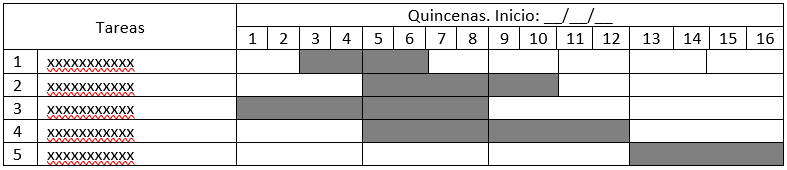
\includegraphics[scale=.8]{./crono_tareas}
\end{center}
\end{table}
\end{center}

\subsection{Operacionalización de variables}
En esta subsección se deben identificar las variables con que se manifiesta el fenómeno objeto de investigación. Seguidamente, las variables deben ser operacionalizadas, ya que se debe operar con ellas, vale decir, se las debe estimar para así conocer cómo se manifiesta el fenómeno. Es importante seleccionar correctamente para incluir todas las variables que son claves según el enfoque con que se aborda la solución del problema de investigación, pero que sean pocas para facilitar su control.

La operacionalización de variables conlleva proveer, en párrafo separado para cada variable, su: a) Denominación: una palabra o frase que identifique lo más precisamente posible la variable. b) Definición: breve explicación descriptiva del significado de la variable. Y c) Estimador: se debe indicar el modo de estimar la variable; puede ser una unidad de medida, típicamente para variable cuantificable, ej. \textit{voltio}; un instrumento o una escala definida, típicamente para variables cualitativas, ej. \textit{métrica de calidad de software}, \textit{escala Likert sobre grado de satisfacción con el aplicativo, criterio de experto sobre la configuración del sistema, descripción técnica de parámetros del transformador de potencia, ...} Las partes descriptivas a), b) y c) deben escribirse en oraciones simples separadas por punto y seguido. Para este efecto hay que seguir el formato de la lista mostrada a continuación.

\begin{enumerate}
\item Nombre de la variable 1: Definición de la variable 1. Estimador de la variable 1.
\item Nombre de la variable 2: Definición de la variable 2. Estimador de la variable 2.\\
 $ \vdots $
\item Nombre de la variable \textit{n}: Definición de la variable \textit{n}. Estimador de la variable \textit{n}.
\end{enumerate}

Luego de haber definido y operacionalizado todas las variables, se debe elaborar y desplegar una tabla, como la tabla \ref{tab:opera} en la que deben aparecer de izquierda a derecha: los objetivos específicos en la primera columna, y yuxtapuestos en las columnas aledañas, para cada objetivo por separado, a partir de la segunda columna, respectivamente: las tareas que conlleva lograr el objetivo, las variables de trabajo que serán estimadas para conocer cómo se resuelve el objetivo, y en la última columna, el estimador unívoco para la variable. El epígrafe de tabla debe situarse sobre la tabla, como se muestra en la tabla \ref{tab:opera}.

\begin{center}
\begin{table}[h]
\begin{center}
\caption{Operacionalización de variables.}\label{tab:opera}
\begin{tabular}{||l|l|l|r||}
\hline
\cellcolor{gray!25} Objetivo específico& \cellcolor{gray!25} Tarea & \cellcolor{gray!25} Variable &\cellcolor{gray!25} Estimador*\\
\hline
\multirow{2}{*}{Objetivo 1}&''&''&''\\
&''&''&''\\
\hline
\multirow{2}{*}{Objetivo 2}&''&''&''\\
&''&''&''\\
\hline
\multirow{2}{*}{Objetivo 3}&''&''&''\\
&''&''&''\\
\hline
\multicolumn{4}{||c||}{{\scriptsize *Estimador: unidad de medida o instrumento, o especie de indicador descriptor de la variable.}}\\
\hline
\end{tabular}
\end{center}
\end{table}
\end{center}

Si la tarea de construir tabla en Latex se vuelve compleja y ardua, se la puede construir en algún editor de preferencia y luego guardarla como imagen de tabla en archivo png, jpg o pdf, en el mismo directorio o carpeta del archivo tex del PTFG, como es el caso de la tabla \ref{tab:opera_2}. Como se puede apreciar, el entorno que contenga la tabla debe ser \textit{$\backslash$begin$\lbrace$table$\rbrace$ ... $\backslash$end$\lbrace$table$\rbrace$}, para que el contador de tablas la considere tabla.

\begin{center}
\begin{table}[H]
\begin{center}\caption{Imagen de tabla empleada en lugar de tabla.\label{tab:opera_2}}
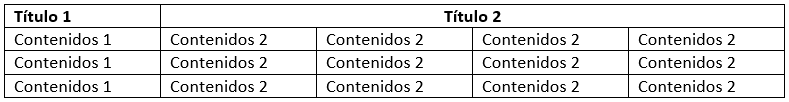
\includegraphics[scale=.8]{./operac}
\end{center}
\end{table}
\end{center}

\textbf{\textit{Elementos gráficos.}} Son útiles para ayudar a ilustrar conceptos, relaciones y todo tipo de resultado desplegable como imagen visual. Entre estos elementos resalta por su importancia el diagrama de flujo del método del trabajo, en general; y en particular, el diagrama funcional del producto del trabajo. Un diagrama funcional es aquel que muestra las funciones de un sistema de forma gráfica y con algunas aclaraciones, es decir, con referencia cruzada en el texto, como este diagrama de la figura \ref{fig:diagrama}. El epígrafe de figura debe situarse al pie de la figura, como se muestra en la figura \ref{fig:diagrama}.

\begin{figure}[H]
\begin{minipage}{\textwidth}
\begin{center}
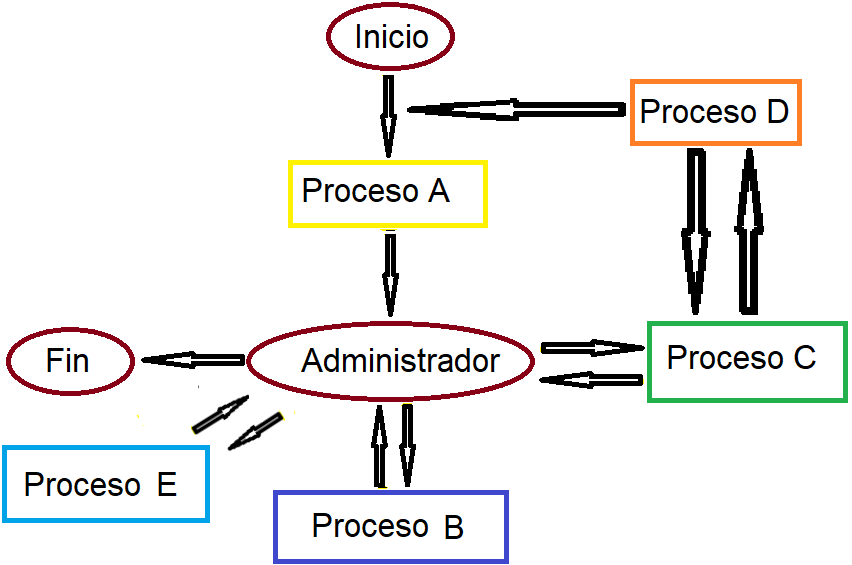
\includegraphics[scale=.5]{./diag_funcional}
\caption{Diagrama funcional}
\label{fig:diagrama}
\end{center}
\end{minipage}
\end{figure}

\textbf{\textit{Entornos matemáticos.}} Las expresiones matemáticas se escriben solamente dentro de entornos matemáticos, también, en general, los símbolos propios de expresiones matemáticas. A continuación, algunos de estos entornos y expresiones matemáticas como ejemplos:

Una ecuación en línea puede escribirse de esta manera: $\int_{-\infty}^{\infty} e^{-x^{2}} \, dx
= \sqrt{\pi}$, donde el entorno en línea está denotado por el par de apertura y cierre \$ \dots \$. Opcionalmente, se logra el mismo resultado con el par $ \backslash( \dots \backslash) $, como puede apreciarse: \( \int_{-\infty}^{\infty} e^{-x^{2}} \, dx
= \sqrt{\pi} \).

Una expresión matemática desplegada en línea especial separada del texto se obtiene con el entorno matemático creado por el par de apertura y cierre $ \backslash[ \dots \backslash] $. Por ejemplo: \[ \left( \frac{1}{2} \right)^{\alpha} \] se obtiene de esta manera.

Cuando se demanda de ecuaciones numeradas, principalmente útiles para referencias cruzadas a las mismas, se emplea el siguiente entorno matemático que produce la salida correspondiente:

\begin{equation}
\sum_{i = 1}^{ \left[ \frac{n}{2} \right] }
\binom{ x_{i, i + 1}^{i^{2}} }
{ \left[ \frac{i + 3}{3} \right] }
\frac{ \sqrt{ \mu(i)^{ \frac{3}{2}} (i^{2} - 1) } }
{\sqrt[3]{\rho(i)-2} + \sqrt[3]{\rho(i) - 1}}
\end{equation}

Nótese el uso de indentación jerárquica para rastrear la estructura de la fórmula, el espaciado para resaltar las llaves y la separación de líneas para los varios pedazos de fórmulas que son más largas que una línea de texto normal. Latex posee la capacidad de gestión automática de numeración y contadores, de manera que el escritor no debe actualizar manualmente los cambios de número y sus respectivas referencias.

Como ejemplo final, este es un ejemplo de referencia cruzada, (teorema \ref{Pitag} y Ec. \ref{pitag}):

\begin{teorema}[Teorema de Pitágoras]
En un triángulo rectángulo, el cuadrado de la hipotenusa es igual a la suma de los cuadrados de los catetos:
\begin{equation}
hip^2 = cat_1^2 + cat_2^2
\label{pitag}
\end{equation}
\label{Pitag}
\end{teorema}
donde: \textit{hip} es la hipotenusa del triángulo rectángulo y, $ cat_1 $ y $ cat_2 $ son los catetos del mismo.

\addcontentsline{toc}{section}{Referencias Bibliográficas}

\bibliographystyle{IEEEtran-castellano}
\bibliography{refer}

\end{document}